\section{Control Methods}%
\label{sec:control_methods}
This section elaborates on why control is required and which control methods are best suitable for various control applications. Predictive control methods have been selected from many control methods because they heavily rely on a dynamic model of the system they control. During this thesis, the effect of the robot interacting with objects is captured by dynamic system models. In addition to predicting output with system models, predictive control methods use the system models to determine action input. A requirement for a controller is that it should yield a stable closed-loop control because that guarantees converging toward a set point. In the proposed framework, controllers are later selected for yielding desired metrics grouped in \Cref{sec:monitoring_metrics}. The two control methods that are used during testing are discussed below.\bs

\paragraph{\acl{MPC}}
The basic concept of \ac{MPC} is to use a dynamic model to forecast system behaviour and optimize the forecast to produce the best decision for the control move at the current time. Models are central to every form of \ac{MPC}~\cite{rawlings_model_2020}. A dynamical model can be presented in various forms, let's consider a familiar differential equation.
$$ \frac{dx}{dt} = f(x(t), u(t)) $$
$$ y = h(x(t), u(t)) $$
$$ x(t_0) = x_0 $$

In which $x \in \mathbb{R}^n $ is the state, $u \in \mathbb{R}^m$ is the input, $y \in \mathbb{R}^p$ is the output, and $t \in \mathbb{R}$ is time. The initial condition specifies the value of the state $x$ at $t = t_0$, and a solution to the differential equation for time greater than $t_0$, $t \in \mathbb{R}_{\geq 0}$ is sought. If little knowledge about the internal structure of a system is available, it may be convenient to take another approach where the state is suppressed, no internal structure about the system is known and the focus lies only on the manipulable inputs and measurable outputs. As shown in \cref{figure: mpc_block_diagam}, consider the system $G(t)$ to be
the connection between $u$ and $y$. In this viewpoint, various system identification techniques are used, in which $u$ is manipulated and $y$ is measured~\cite{rawlings_model_2020}. From the input-output relation, a system model is estimated or improved. The system model can be seen inside the \ac{MPC} controller block in \cref{figure: mpc_block_diagam}.\\

\begin{figure}[H]
\centering
\begin{tikzpicture}
% blocks
\node[draw,
    minimum width=2cm,
    minimum height=1.2cm,
    fill=myLightColor,
] (system) at (0,0){$G(t)$};
\node[draw,
    minimum width=5.5cm,
    minimum height=2cm,
    fill=myEvenLighterColor,
    below = 1cm of system,
    label=above:MPC controller,
] (controller) {};
% the blocks and arrows inside MPC
\node[draw, minimum width=2cm, below=3mm of controller.north, anchor=north, fill=myDarkColor] (optimisation) {Optimisation};
\node[draw, below=8mm of optimisation.south, anchor=south, fill=myDarkColor] (model) {System Model};
\path[-stealth]
        (model.east) edge[bend right=70] node[pos=0.5, right] {Predict} (optimisation.east)
        (optimisation.west) edge[bend right=70] node[pos=0.5, left] {Action}  (model.west);
% Arrows
\draw[-stealth] (controller.west) |- ($(controller.west) - (1,0mm) $) |- (system.west)
node[near end, above]{$u(t)$};
\draw[stealth-] ([yshift=-0.3cm]controller.east) -- ++(3,0) node[midway, above](input){$y_{ref}(t)$, $p$, $\mathbb{X}$, $\mathbb{U}$, $\mathbb{Y}$};
\draw[-stealth] (system.east) -- ++ (5, 0)
    node[midway](output){}node[midway,above]{$y(t)$};
    \draw [-stealth] (output.center) |- ([yshift=0.5cm]controller.east);
\end{tikzpicture}
\caption{System $G(t)$ with input ${u}(t)$, output $y(t)$ and \acs{MPC} controller with input $y(t)$\\reference signal $y_{ref}(t)$, parameterisation $p$ and constraint sets $\mathbb{X}$, $\mathbb{U}$, $\mathbb{Y}$} \label{figure: mpc_block_diagam} \end{figure}

Some states of the system might be inside an obstacle region, such a region is undesirable for the robot to be in or go toward. The robot states are allowed in free space, which is all space minus the obstacle region. The free space is specified as a state constrained set $\mathbb{X}$. Allowable input can be restricted by the input constraint set $\mathbb{U}$, a scenario in which input constraints are required is for example the maximum torque an engine produces at full throttle. Lastly, the set of allowed outputs is specified in the output constraint set $\mathbb{Y}$. State, input and output constraints must be respected during optimisation, the optimiser takes the state-, input- and output constraint sets $\mathbb{X}$, $\mathbb{U}$, $\mathbb{Y}$ and if feasible, finds an action sequence driving the system toward the reference signal while constraints are respected. The \ac{MPC} system model predicts future states where the system is steered toward as a result of input actions.\\

The optimisation minimises an objective function $V_{N}(x_{0}, y_{ref}, \mathbf{u}_{N}(0))$, where\\ $ \mathbf{u}_{N}(k) = (u_k, u_{k+1}, \dots , u_{k+N})$. The objective function takes the reference signal as an argument together with the initial state and the control input for the control horizon. The objective function then creates a weighted sum of some heuristic function. States and inputs resulting in outputs far from the reference signal are penalised more by the heuristic function than outputs closer to the reference signal. Because the objective function is a Lyapunov function, it has the property that, it has a global minimum for the optimal input $\mathbf{u}_{N}^*$. If the system output reaches the reference signal $y_{ref}$, $x_{ref}$ then $u_{ref}$ will be mapped to the output reference signal as such $y_{ref} = h(x_{ref}, u_{ref})$. As a result solving the minimisation problem displayed in \cref{equation: mpc_problem} gives the optimal input which steers the system toward the output reference signal while at the same time respecting the constraints.

\begin{mini}
{u_k, u_{k+1}, \dots , u_{k+N}} {
V_{N}(x_{0}, y_{ref}, u_k, u_{k+1}, \dots , u_{k+N})
}
{}{}
\addConstraint{x(k+1) = f(x(k), u(k))}
\addConstraint{x \in \mathbb{X}}
\addConstraint{u \in \mathbb{U}}
\addConstraint{y \in \mathbb{Y}}
\addConstraint{x(0) = x_0}
\label{equation: mpc_problem}
\end{mini}

After solving the minimisation problem, \cref{equation: mpc_problem}, the optimal input sequence is obtained $\mathbf{u}^*_N$ (given that the constraints are respected for such input), from which only the first input is executed for time step $k$ to $k+1$. Then all indices are shifted such that the previous time step $k+1$ becomes $k$, the output is measured and the reference signal, parameterisation, and constraints sets are updated and a new minimisation problem is created, which completes the cycle.\bs

\paragraph{\acl{MPPI} Control}
Introduced by~\cite{williams_model_2015} \ac{MPPI} control arose, which was followed by \ac{MPPI} control combined with various system identification methods and system models~\cite{abraham_modelbased_2020,cong_selfadapting_2020,arruda_uncertainty_2017}. The core idea is from the current state of the system with the use of a system model and randomly sampled inputs to simulate in the future a number of "rollouts" for a specific time horizon,~\cite{neuromorphictutorial_ltc21_2021}. These rollouts indicate the future states of the system if the randomly sampled inputs would be applied to the system, the future states can be evaluated by a cost function which penalised undesired states and rewards desired future states. A weighted sum over all rollouts determines the input which will be applied to the system. If a goal state is not reached, the control loop starts with the next iteration. An example is provided, see  \cref{figure: mppi_car_with_rollouts}.

\begin{figure}[H]
    \centering
    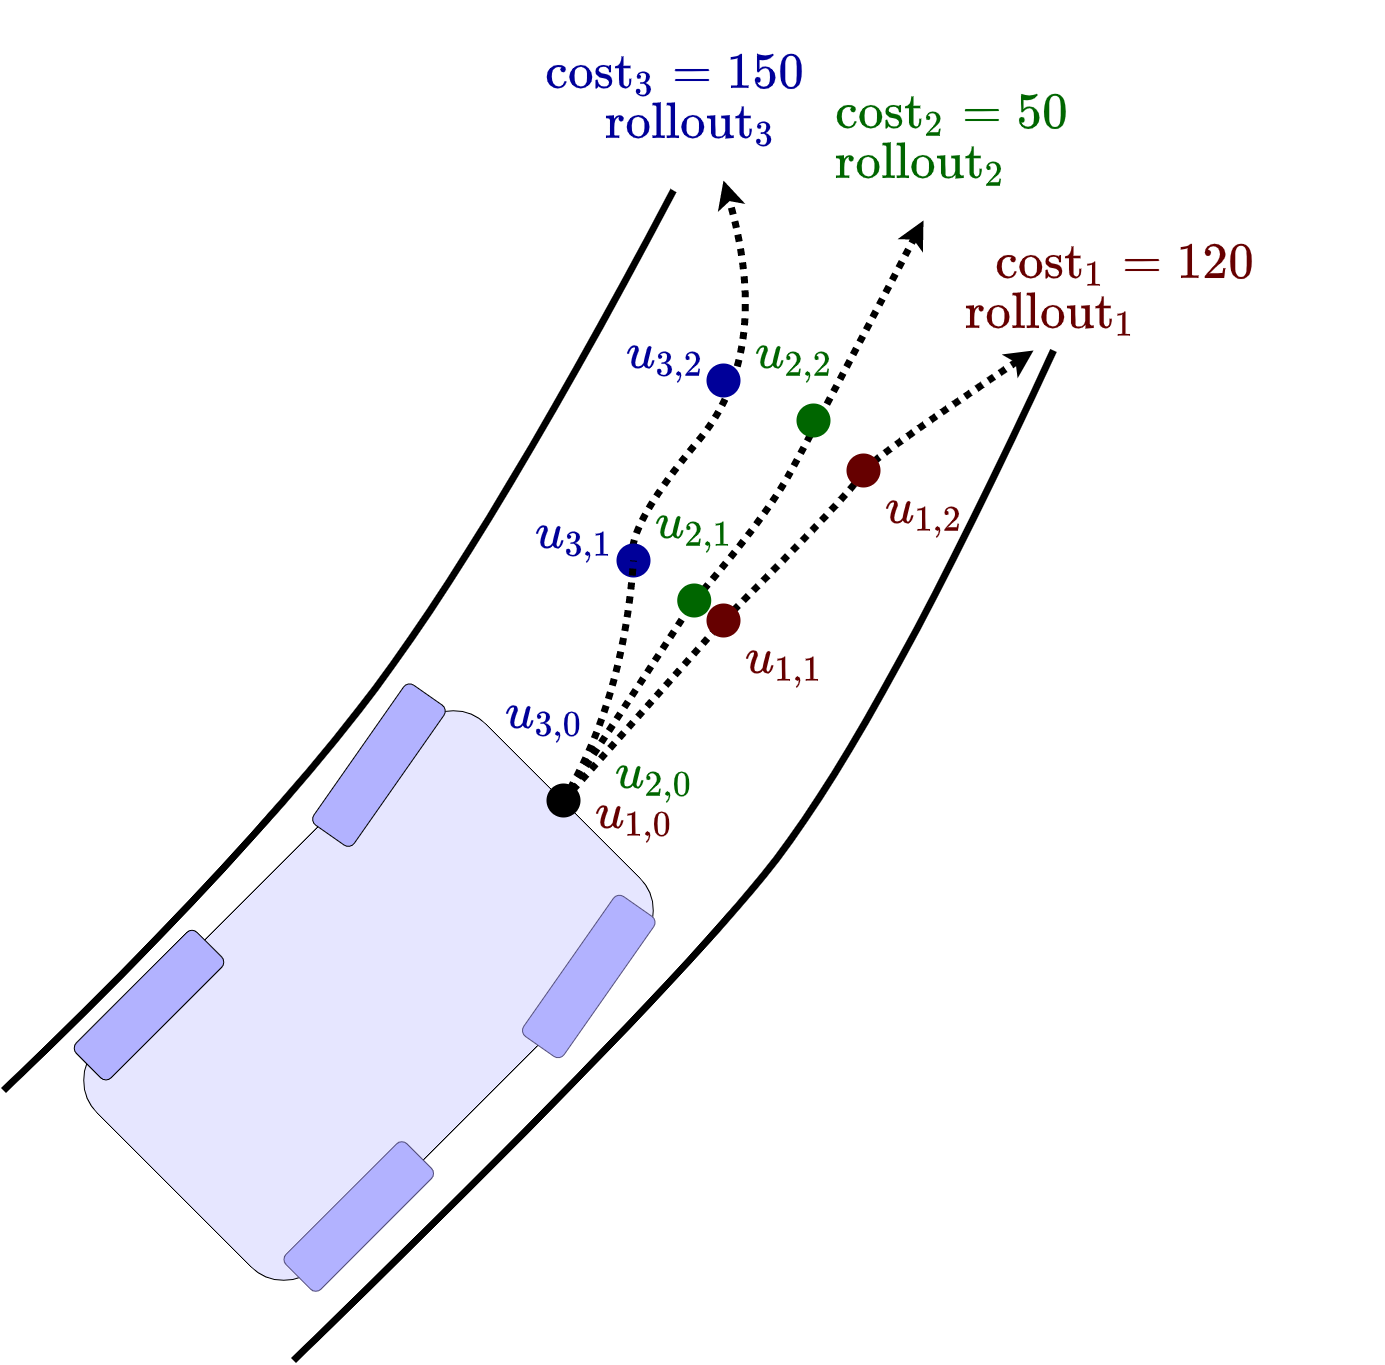
\includegraphics[width=0.5\textwidth]{figures/appendix/MPPI_car_with_rollouts.png}
    \caption{\acs{MPPI} controlled race car using a control horizon of 3 time steps, with 3 rollouts all having their respected inputs as $u_{i,j}$ where $i$ is the rollout index and $j$ indicates the time step~\cite{neuromorphictutorial_ltc21_2021}.}
    \label{figure: mppi_car_with_rollouts}
\end{figure}

Here 3 rollouts are displayed, The objective function is designed to keep the car driving on the center of the road by penalising rollouts which are further away from the center of the road relatively more. resulting in a high cost for $\text{rollout}_1$ and $\text{rollout}_3$ compared to $\text{rollout}_2$. As a result, the input send to the system as a weighted sum of the rollouts is mostly determined by $\text{rollout}_2$. The weighted sum determining the input is displayed in \cref{equation: mppi_weighted_sum}, from~\cite{neuromorphictutorial_ltc21_2021}.

\begin{equation}
u(k+1)=u(k)+\frac{\sum_{i} w_{i} \delta u_{i}}{\sum_{i} w_{i}}
\label{equation: mppi_weighted_sum}
\end{equation}

Where $\delta u_i$ is the difference between $u(k)$ and the input for rollout $i$, the weight of $\text{rollout}_i$ is detemined as: $w_{i}=e^{-\frac{1}{\lambda} \text{cost}_{i}}$, $\lambda$ is a constant parameter.\bs


The core idea is from the current state of the system using a system model and randomly sampled inputs to simulate several \quotes{rollouts} for a specific time horizon,~\cite{neuromorphictutorial_ltc21_2021}. These rollouts indicate the system's future states if the randomly sampled inputs are applied. The future states can be evaluated by a cost function penalizing undesired states and rewarding desired future states. A weighted sum over all rollouts determines the input which will be applied to the system. The main advantage \ac{MPPI} has over \ac{MPC} control is that it is better suited for nonlinear system models. Whilst linear models can accurately estimate drive applications, push applications are harder to estimate with a linear model. Thus \ac{MPPI} is selected mainly for push applications.\bs

The properties of \ac{MPC} suggest that it is best suitable for drive actions because of easy tuning and robustness. \Ac{MPPI} control is compatible with nonlinear system models, making it more suitable for push actions. It is worth mentioning that the goal of this thesis is not to find the best optimal controller. The goal is to gradually, over time, choose control methods in combination with system models that result in better performance, and the performance is measured with various metrics, discussed in \Cref{chap:h-graph_and_k-graph}.\bs
